\documentclass{article}
\usepackage[catalan]{babel}
\usepackage[latin1]{inputenc}   % Permet usar tots els accents i car�ters llatins de forma directa.
\usepackage{enumerate}
\usepackage{amsfonts, amscd, amsmath, amssymb}
\usepackage[pdftex]{graphicx}
\usepackage{longtable}

\setlength{\textwidth}{16cm}
\setlength{\textheight}{24.5cm}
\setlength{\oddsidemargin}{-0.3cm}
\setlength{\evensidemargin}{0.25cm} \addtolength{\headheight}{\baselineskip}
\addtolength{\topmargin}{-3cm}

\newcommand\Z{\mathbb{Z}}
\newcommand\R{\mathbb{R}}
\newcommand\N{\mathbb{N}}
\newcommand\Q{\mathbb{Q}}
\newcommand\K{\Bbbk}
\newcommand\C{\mathbb{C}}
\newcommand\cT{{\cal T}}
\def\fl{\text{fl}}
\def\pt{\text{pt}}
\def\fm{\text{fm}}

\newcounter{exctr}
\newenvironment{exemple}
{ \stepcounter{exctr} 
\hspace{0.2cm} 
\textit{Exemple  \arabic{exctr}: }
\it
\begin{quotation}
}{\end{quotation}}


\begin{document}

\begin{center}
\textbf{\Large Processament Digital del Senyal \\ Enginyeria T�cnica en Telem�tica \\ Examen Juny 2011}
\end{center}

\begin{description}

\item[Problema 1]. 

\begin{enumerate}[a)]

\item Raonau si un sistema LTI queda determinat coneixent la resposta que d�na quan s'excita
amb l'esgla� unitari $u[n]$.
\ \hfill{\textbf{ 4 pt.}}

\item Donat l'esquema de la figura seg�ent:

\begin{center}
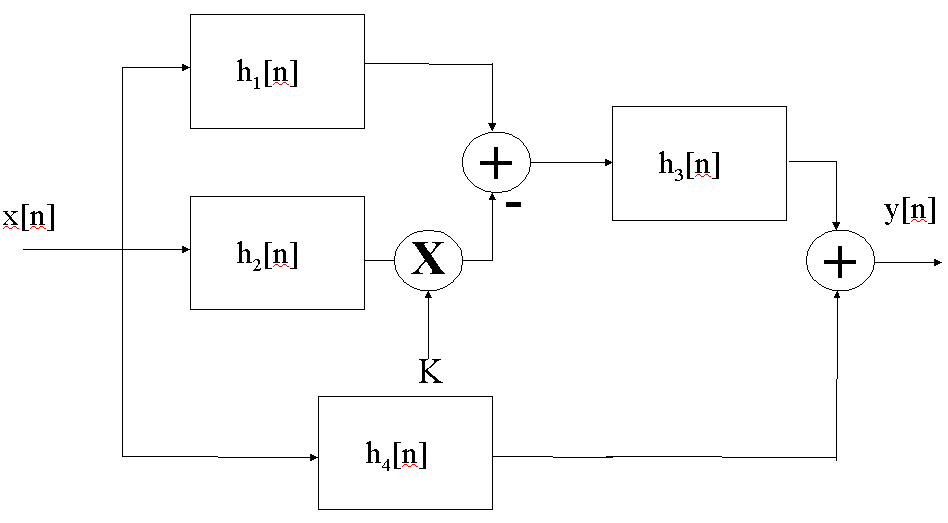
\includegraphics[width=10cm]{esquemaP1.png}
\end{center}

\noindent
on $h_1[n]=2 (\frac{1}{2})^n u[n]$, $h_2[n]=h_1[n-4]$, $h_3[n]=\{ \underline{-1}, 0, 1 \}$
i $h_4[n]=\{ \underline{0}, a, \frac{1}{2}, b, 0, c \}$.

\vskip 0.3 cm
\noindent
Trobau els valors de les constants $K$, $a$, $b$ i $c$ que fan que el sistema es comporti com
un filtre FIR de fase lineal generalitzada de tipus II.

\ \hfill{\textbf{ 6 pt.}}

\end{enumerate}

\vskip 1cm


\item[Problema 2].
Un mateix senyal $x[n]$ s'aplica a tres sistemes LTI causals com a la figura seg�ent:

\begin{center}
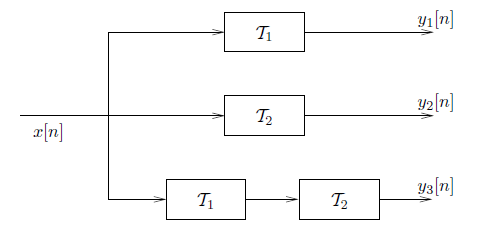
\includegraphics[width=10cm]{esquemaP2.png}
\end{center}

\noindent
Sabent que
\[
\begin{array}{l}
y_1[n]=(0.5)^n u[n]+(-0.5)^n u[n], \\ 
y_2[n]=9 (0.4)^n u[n], \\ 
y_3[n]=10 (-0.5)^n u[n] + 8 (0.4)^n u[n]
\end{array}
\]

\noindent
\begin{enumerate}[a)]
\item Calculau les transformades ${\cal Z}$ del senyal d'entrada $x[n]$ i 
de les respostes impulsionals $h_1[n]$ i $h_2[n]$ 
dels sistemes ${\cal T}_1$ i  ${\cal T}_2$.
 \ \hfill{\textbf{ 4 pt.}}
\item Trobau el senyal $x[n]$ i les respostes impulsionals $h_1[n]$ i $h_2[n]$ 
dels sistemes ${\cal T}_1$ i  ${\cal T}_2$.
 \ \hfill{\textbf{ 4 pt.}}
\item Discutiu l'estabilitat dels sistemes $h_1[n]$ i $h_2[n]$.
 \ \hfill{\textbf{ 2 pt.}}
\end{enumerate}
  
  

\vskip 1cm

\item[Problema 3].
Considerau el sistema digital de processament del senyal anal�gic de la figura seg�ent:


\begin{center}
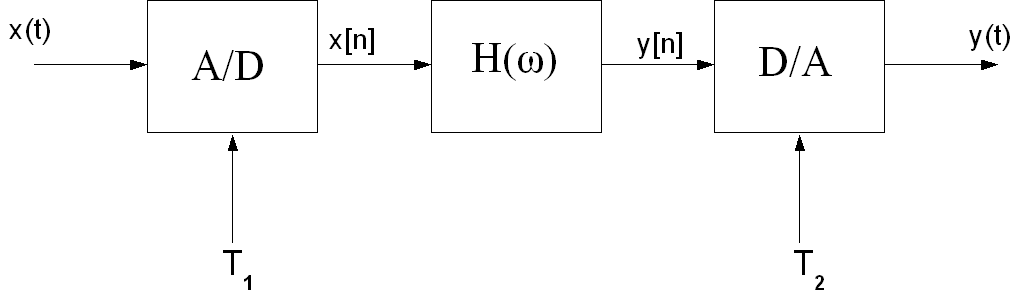
\includegraphics[width=10cm]{esquemaADDAT1T2.png}
\end{center}

\begin{center}
\begin{tabular}{cc}
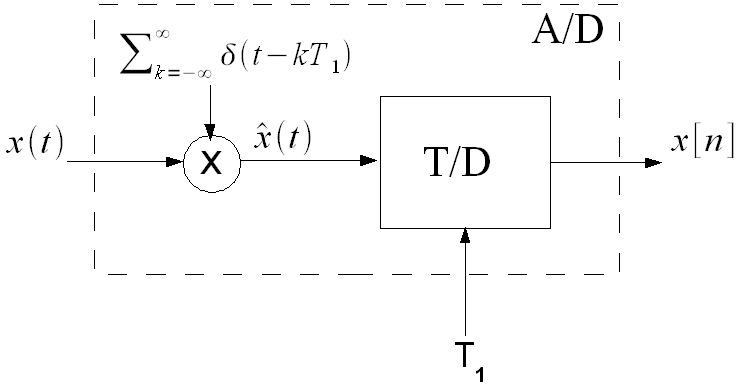
\includegraphics[width=6cm]{ADT1.png}
&
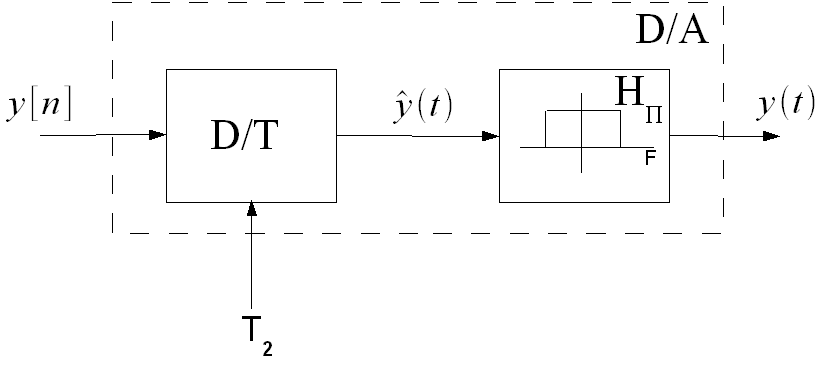
\includegraphics[width=6cm]{DAT2.png}
\end{tabular}
\end{center}

\noindent
El filtre digital $H(\omega)$ est� definit de la seg�ent manera:
$
H(\omega)=\begin{cases} 1 & \text{si } \omega_1 \leq | \omega | \leq \omega_2 \\ 0 & \text{resta} \end{cases}
$

\noindent
L'espectre del senyal d'entrada �s:
\begin{minipage}{6cm}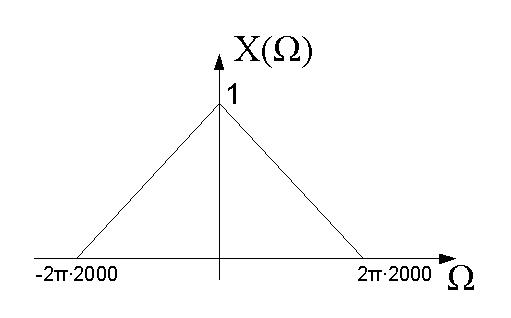
\includegraphics[width=6cm]{inputP3.png}\end{minipage} 

\noindent
Un agent secret oculta un missatge en el rang de freq��ncies $[1000, 1500]$ Hz del senyal d'entrada.
Responeu raonadament les seg�ents q�estions:


\begin{enumerate}[a)]
\item Calculau $T_1$ sabent que �s el m�xim periode de mostreig que permet recuperar el missatge ocult
(es permet aliasing a la resta del senyal d'entrada).
 \ \hfill{\textbf{ 2 pt.}}
\item Calculau els par�metres del filtre digital $H(\omega)$ ($\omega_1$ i $\omega_2$) que permet  
recuperar el missatge ocult i elimina la resta del senyal d'entrada.
 \ \hfill{\textbf{ 2 pt.}}
 \item Calculau el valor de $T_2$ que permet recuperar el missatge ocult en el rang de freq��ncies $[100, 150]$ Hz 
 \ \hfill{\textbf{ 2 pt.}}
\item Dibuixau l'espectre de tots els senyals
que intervenen en el sistema: $\hat{x}(t)$, $x[n]$, $y[n]$, $\hat{y}(t)$ i $y(t)$.
\newline
. \ \hfill{\textbf{ 4 pt.}}

\end{enumerate}

\vskip 1cm

\item[Problema 4].

\begin{enumerate}[a)]
\item Determinau la magnitud i la fase  de $H(\omega)$ per al filtre seg�ent:  
$h[n]=\{ \underline{1}, \frac{7}{2}, \frac{7}{2}, 1 \}$
. \ \hfill{\textbf{ 2 pt.}}

\item Per al filtre de l'apartat anterior
determinau la sortida quan l'entrada �s
\[
x[n]=5 - \frac{2}{3} \cos ( \frac{5 \pi}{4} n + \frac{\pi}{3} ))
\]
 \ \hfill{\textbf{ 2 pt.}}
 

\item Trobau la resposta impulsional dels dos possibles
sistemes FIR reals de fase lineal generalizada que tenen un zero a $z=2$
i que prenen valors entre $n=0$ i $n=3$. Dibuixau els seus diagrames de pols i zeros.
 \ \hfill{\textbf{6 pt.}}



\end{enumerate}

\end{description}

\vskip 1cm

\noindent
Duraci� de l'examen: 4 hores.



\end{document}
